\documentclass[tikz,border=6pt]{standalone}
% Shared style for the HERMESS schematic figures (compiled by build.sh).
% ETH palette; Latin Modern (the LaTeX default) to match the documentation.
\usepackage{amsmath}
\usepackage{tikz}
\usetikzlibrary{arrows.meta,positioning,calc,shapes.geometric,circuits.ee.IEC}
\definecolor{ethblue}{HTML}{215CAF}
\definecolor{ethpetrol}{HTML}{007894}
\definecolor{ethgrey}{HTML}{6F6F6F}
\tikzset{
  block/.style      = {draw=ethblue, thick, fill=ethblue!8, minimum height=9mm,
                       minimum width=16mm, inner sep=2.5pt, align=center},
  sum/.style        = {draw=ethblue, thick, circle, fill=white, minimum size=4.5mm, inner sep=0pt},
  sig/.style        = {-{Latex[length=2.4mm]}, thick},
  wire/.style       = {thick},
  node distance     = 9mm and 12mm,
  every node/.style = {font=\small},
  lbl/.style        = {font=\small, inner sep=1.5pt},
  port/.style       = {font=\small\itshape, text=ethgrey},
}

\begin{document}
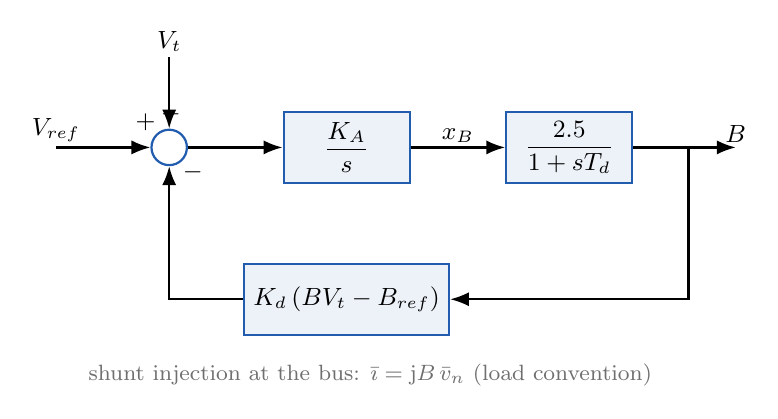
\begin{tikzpicture}
  \node[sum] (s) {};
  \node[lbl] at ($(s)+(-0.30,0.32)$) {$+$};
  \node[lbl] at ($(s)+(0.02,0.42)$)  {$-$};
  \node[lbl] at ($(s)+(0.30,-0.32)$) {$-$};
  \node[block, right=of s, minimum width=16mm] (ka) {$\dfrac{K_A}{s}$};
  \node[block, right=12mm of ka] (lag) {$\dfrac{2.5}{1 + sT_d}$};
  \coordinate[left=12mm of s] (in);
  \draw[sig] (in) node[above, lbl] {$V_{ref}$} -- (s);
  \draw[sig] ($(s)+(0,1.15)$) node[above, lbl] {$V_t$} -- (s);
  \draw[sig] (s) -- (ka);
  \draw[sig] (ka) -- (lag) node[midway, above, lbl] {$x_B$};
  \draw[sig] (lag.east) -- ++(1.3,0) node[above, lbl] {$B$};
  % droop feedback
  \node[block, below=10mm of ka, minimum width=26mm] (droop) {$K_d\,(B V_t - B_{ref})$};
  \draw[sig] ($(lag.east)+(0.7,0)$) |- (droop.east);
  \draw[sig] (droop.west) -| (s);
  \node[lbl, text=ethgrey] at ($(droop.south)+(0.3,-0.5)$)
    {\footnotesize shunt injection at the bus: $\bar{\imath} = \mathrm{j}B\,\bar v_n$ (load convention)};
\end{tikzpicture}
\end{document}
